\documentclass[11pt]{article}
\usepackage[letterpaper,margin=1in]{geometry}
\usepackage[T1]{fontenc}
\usepackage[utf8]{inputenc}
\usepackage{lmodern}
\usepackage{microtype}
\usepackage{graphicx}
\usepackage{booktabs}
\usepackage{array}
\usepackage{float}
\usepackage{pdflscape}
\usepackage[font=small,labelfont=bf]{caption}
\usepackage{xurl}
\usepackage[hidelinks]{hyperref}
\graphicspath{{figures/}}
\setlength{\parindent}{1em}
\setlength{\parskip}{0.25em}
\setlength{\emergencystretch}{3em}
\title{NeuroSelect: A Reproducible Offline Framework for Profile-Conditioned Language Ranking and Counterfactual P300 Candidate Fusion}
\author{Nick Somitsch}
\date{}

\begin{document}
\maketitle

\begin{abstract}

\textbf{Background:} Language prediction can reduce the number of explicit selections required by a brain-computer interface (BCI), but a language model can rank an intended continuation only when that continuation is present in the visible candidate set. Studies that report ranking conditionally on candidate availability can therefore obscure a more basic coverage bottleneck.


\textbf{Objective:} We developed NeuroSelect, a reproducible offline framework that keeps candidate generation, language ranking, P300 decoding, retrieval, fusion, and confirmation as separately auditable components. We asked whether profile-specific language adapters improve ranking on held-out synthetic messages, how a classical and a neural decoder perform on held-out public P300 data, whether fused evidence improves a counterfactual replay, and whether compositional candidate interfaces mitigate observed opening failures.


\textbf{Methods:} Four fixed synthetic profiles contributed \textbf{3,990 held-out next-span trials from 1,000 messages}. A pinned four-bit Qwen3-4B model generated target-blind candidates, and four independently trained low-rank adapters rescored fixed candidate sets. Public bigP3BCI Study P data were split by participant into training, validation, and test partitions. A calibrated xDAWN-LDA decoder and a secondary EEGNet comparator were evaluated on the original target/non-target flash task. Recorded held-out P300 probabilities were then remapped to synthetic candidate menus in a balanced offline counterfactual replay. Exploratory experiments tested grammar/profile ablations and one-, two-, and three-stage opening composition.


\textbf{Results:} The frozen language generator made the intended span available in \textbf{28.7\% of trials (95\% CI 27.3\%-30.1\%)}, and complete-message availability was \textbf{0.0\%}. Conditional on availability, personalization improved top-1 recall by \textbf{9.6 percentage points (95\% CI 6.4-12.9)} overall, but reduced it by \textbf{9.1 points (95\% CI 2.9-15.2 reduction)} for the concise profile. On \textbf{21,491 held-out labeled epochs}, xDAWN-LDA achieved \textbf{AUROC 0.800} and \textbf{Brier score 0.062}. EEGNet had no clearly established selection-ranking advantage and a \textbf{0.089 higher Brier score (95\% CI 0.084-0.095)}. In counterfactual replay, the complete system changed top-1 recall by \textbf{+0.7 percentage points (95\% CI 0.0-2.8)} and completion by \textbf{0.0 points} relative to BCI-only replay. Exploratory target-blind generation increased span availability to \textbf{52.5\%}, while three-stage composition covered \textbf{66.7\%} of unseen combinations of observed components but \textbf{0.0\%} of openings from unseen paraphrase families.


\textbf{Conclusions:} NeuroSelect provides a checksum-addressed way to study language-assisted P300 candidate selection without merging unlike evidence tiers. The experiments identify candidate coverage, especially message openings and unseen surface families, as the largest observed bottleneck in the evaluated pipeline. They do not demonstrate live communication benefit, clinical efficacy, or open-vocabulary thought decoding.


\textbf{Keywords:} brain-computer interface; P300; language prediction; personalization; candidate generation; counterfactual replay; reproducible research.


\end{abstract}

\section{Introduction}

Brain-computer interfaces create a non-muscular control channel from measured neural activity to an external device \cite{wolpaw2002}. The P300 matrix speller is a canonical non-invasive example: a user attends to a desired item while rows, columns, or individual stimuli flash, and target flashes elicit event-related activity that can be distinguished from non-target flashes \cite{farwell1988}. Many variants have since changed stimulus design, classification, stopping rules, and the displayed symbol set \cite{rezeika2018,pan2022}. Despite these advances, spelling remains a sequence of costly explicit selections. Language information is consequently attractive because it can raise the prior probability of plausible continuations or expose multiword candidates. Earlier offline P300 work showed that integrating natural-language probabilities with dynamic classification can improve character-level accuracy and bit rate \cite{speier2012}.


Predictive-language integration has also been evaluated in online P300 spelling. A predictive-word interface reduced task-completion time but also reduced accuracy \cite{ryan2011}, while a trigram language model incorporated into online dynamic stopping reduced the required data collection and increased communication rate under its tested protocol \cite{mainsah2014}. More recently, offline simulations have compared GPT-2, BERT, and BART language components for P300 spelling and reported model-dependent typing-speed estimates \cite{parthasarathy2024}. Those studies primarily addressed character or word prediction and communication-rate simulation. NeuroSelect instead isolates exact phrase-candidate coverage, conditional ranking, original-task EEG decoding, and counterfactual phrase-menu replay so that performance at one layer is not treated as evidence at another.


Moving from character priors to generated phrase menus creates a different failure mode. Let an intended next span be $y$, a target-blind generator produce a finite candidate set $C(x)$ from context $x$, and a ranker order the members of that set. Ranking quality is relevant only when $y \in C(x)$. A strong conditional ranker cannot recover an intended continuation that is absent from the interface, and averaging only over available targets can overstate end-to-end usefulness. This distinction is especially important when a compact menu is required for a P300 interface.


Personalization adds a second distinction. A language model adapted to one person's preferred style may alter ranking without improving candidate generation. The effect can also vary by style profile rather than appearing as a uniform gain. Low-rank adaptation (LoRA) offers an efficient way to train separate parameter updates while freezing a common base model \cite{hu2022}, but the resulting adapters should be evaluated on held-out messages and the exact visible candidate set. Retrieval context should likewise remain distinguishable from parametric model adaptation; the present work uses transparent local lexical retrieval rather than treating all contextual augmentation as an undifferentiated model score \cite{lewis2020}.


Evaluating the full interaction poses an additional evidence problem. Public P300 datasets provide recorded neural responses to their original stimuli, not neural responses to newly generated phrase tiles. NeuroSelect therefore separates original-task EEG decoding from counterfactual candidate replay. In the original task, a decoder estimates target/non-target flash probabilities. In the replay, those recorded probabilities are remapped to candidate positions under explicit rules. The remapped words were never selected or endorsed by the source participant. This separation avoids relabeling event discrimination as word-decoding accuracy.


The paper makes three contributions. First, it introduces an offline framework and evidence contract that preserve candidate, language, EEG, retrieval, fusion, and confirmation provenance. Second, it reports frozen component and replay results, including unfavorable coverage and profile-level findings. Third, it uses the failure pattern to motivate explicitly exploratory candidate-generation and hierarchical-opening experiments. The primary research questions concern target availability, conditional personalization, held-out original-task P300 decoding, and prespecified fusion contrasts. The exploratory experiments ask whether known linguistic components can be composed within a fixed candidate budget and where that strategy fails.


The evidence hierarchy is central to interpretation. Synthetic language does not become EEG evidence; original-task EEG does not become message-level communication; counterfactual replay does not become participant use; and developer-authored exploratory benchmarks do not replace the frozen primary result.


\begin{table}[H]
\centering
\caption{Evidence hierarchy and non-pooling boundaries. Every evidence tier is reported separately. No row is a live NeuroSelect user study, and no aggregate "system score" is computed across synthetic language, original-task EEG, counterfactual replay, and exploratory interface experiments.}
\label{tab:table-1-evidence-hierarchy}
\scriptsize
\setlength{\tabcolsep}{3.5pt}
\renewcommand{\arraystretch}{1.15}
\resizebox{\linewidth}{!}{%
\begin{tabular}{@{}lllll@{}}
\toprule
\textbf{Evidence tier} & \textbf{Component} & \textbf{Analysis units} & \textbf{Role} & \textbf{Interpretation limit} \\
\midrule
Primary & Held-out language & 3990 spans / 1000 messages / 4 fixed profiles & Availability and paired ranking & Synthetic teacher-forced language only \\
Primary & xDAWN original-task EEG & 21491 labeled epochs / 3 held-out subjects & Binary decoding and target-event ranking & Occurrence-level Study P events, not symbols \\
Secondary comparator & EEGNet original-task EEG & 21491 identical held-out epochs & Paired model comparison & No clear selection-ranking gain; worse calibration \\
Primary & Counterfactual replay & 144 trials per condition / 3 held-out subjects & Paired fusion and completion contrasts & Offline remapping, not participant use \\
Exploratory test-exposed & Candidate generation v2 & 3990 existing benchmark spans & Target-blind phrase availability & Developer inspected the test benchmark \\
Exploratory locked & Step 4 candidate ablations & 3990 exposed + 4000 combination-holdout spans & Ablations and two-stage interface & Synthetic developer-authored benchmark \\
Exploratory locked & Opening generalization & 288 combinations + 384 unseen-family openings & Hierarchical composition and selection cost & Closed-vocabulary interface evidence \\
\bottomrule
\end{tabular}%
}
\vspace{2pt}
\begin{minipage}{0.98\linewidth}
\footnotesize\textit{Evidence role: evidence-map, primary, primary-with-secondary-comparator, exploratory. Source: checksum-verified publication display.}
\end{minipage}
\end{table}

\section{Materials and methods}

\subsection{Study design and reproducibility contract}

NeuroSelect was evaluated as an offline computational study using synthetic language and secondary analysis of a public P300 dataset. No participant was recruited and no participant used the NeuroSelect interface. The tracked publication protocol fixed five questions, source-run identities, allowed and prohibited claims, and a requirement that weak or null results remain reportable. The primary language, xDAWN-LDA, and counterfactual artifacts existed before that publication protocol and are therefore retrospective evidence. The later candidate-generation and opening-generalization designs are labeled exploratory; their locked or test-exposed status is reported separately.


Every experiment writes a typed result and a checksum-addressed manifest containing the Git revision, configuration digest, dependency versions, hardware summary, input digests, output digests, and random seeds. Manuscript tables and figures are generated only from verified clean manifests. The manuscript assembler verifies the display manifest, all embedded files, references, and a quantitative claim ledger before producing synchronized LaTeX, PDF, Word, and Markdown documents. The LaTeX source and BibTeX bibliography are tracked for journal submission, while the compiled bundle includes the exact publication figures. A dirty source tree can be used for development rendering only and is explicitly marked non-ready. Source code, tests, protocol, analysis recipes, and manuscript sources are maintained in a version-controlled NeuroSelect repository and will be made public with the submission release. Non-restricted result manifests, tables, figures, and publication-analysis outputs will be archived with that release.


\subsection{Synthetic messages and leakage boundaries}

The language benchmark contains four fixed synthetic communication profiles: casual, concise, formal, and reflective. Each profile contributes 250 test messages; across profiles, the frozen test set contains \textbf{1,000 messages}. Each message is segmented into target next spans, producing \textbf{3,990 language trials}. Training, validation, and test messages are disjoint. Profile adapters were optimized only on the corresponding training corpus. Validation loss was monitored during the fixed training schedule, but it was not used for early stopping or best-checkpoint selection. Test loss was evaluated after training, and test messages were then used for the reported ranking benchmark; no test message contributed a training gradient. Because the adapter artifacts existed before the publication protocol was written, these results are retrospective rather than a prospectively sealed evaluation.


Synthetic profiles are controlled style conditions, not people. They contain no private user data and do not establish population generalization. An intended target is used only after generation to compute availability and rank. Generator APIs do not accept the intended target, and artifact checks record this constraint.


Primary next-span contexts were constructed by teacher forcing: after each target span, the next trial context included the preceding reference spans rather than the system's earlier generated or selected output. This isolates per-span candidate generation and ranking from cascading interface errors. Complete-message availability nevertheless required every target span in a message to be available.


\subsection{Candidate generation and language scoring}

The frozen generator used Qwen/Qwen3-4B-MLX-4bit at revision 52a5ab34fa604bc8af6d3ce0cac0cab10b7eb495. Qwen3 is a family of dense and mixture-of-experts language models with support for reasoning and non-reasoning modes \cite{qwen32025}. NeuroSelect disabled thinking, set temperature to zero, allowed at most 512 generated tokens, and limited each visible menu to nine language candidates; three separately scored control actions were handled outside that language-candidate budget. Structured-output validation rejected invalid candidates without inserting the intended answer.


The generic language score is the candidate's mean token log likelihood under the base model. Four profile-specific LoRA adapters were trained independently and verified by checksums before evaluation. The personalized condition rescored the same fixed candidate set; it did not generate a new personalized set. This makes personalization a paired ranking comparison rather than a combined generation-and-ranking intervention. Each adapter used 16 adapted transformer layers, a batch size of one, a learning rate of $10^{-5}$, 600 update iterations, a maximum sequence length of 512 tokens, gradient checkpointing, and seed 20260723. Validation loss was evaluated every 100 iterations; the final scheduled adapter, rather than a validation-selected checkpoint, was used. Training and inference used MLX on Apple silicon \cite{hannun2023}.


For each trial, target availability equals one when the exact intended span occurs in the candidate set. Unconditional top-k recall counts unavailable targets as failures. Conditional top-k recall and reciprocal rank use only available targets. Complete-message availability equals one only when every target span in the message is available. Exact message accuracy additionally requires every target span to be available and ranked first.


\subsection{Public EEG source and preprocessing}

Study P was drawn from bigP3BCI version 1.0.0 on PhysioNet, licensed CC BY 4.0 \cite{mainsah2025}. The release contains \textbf{19 participants and 228 EDF+ spelling-block recordings} from two sessions, acquired with \textbf{32 EEG channels at 256 Hz}. The source task compared predictive and non-predictive 9-by-8 P300 spelling \cite{ryan2011}. NeuroSelect verified source files against the official SHA-256 inventory and retained subject, session, run, condition, flash, target label, and selection-trial provenance.


The model split held out complete participants: \textbf{13 training, 3 validation, and 3 test participants}. Source folders named Train and Test describe task blocks and label availability; they are not model partitions. Only labeled blocks were used for supervised training and evaluation. Test blocks with zero-only label streams were retained as unknown for replay engineering but excluded from supervised denominators.


Preprocessing used MNE-Python \cite{gramfort2013}. The fixed recipe applied a 60-Hz notch filter, 0.5-20-Hz band-pass filter, average reference, epochs from -0.1 to 0.8 seconds, baseline correction from -0.1 to 0 seconds, peak-to-peak artifact rejection, and resampling to 128 Hz. Rejected epochs remained represented in the preprocessing report.


\subsection{Original-task P300 decoders}

The prespecified primary decoder used two xDAWN spatial components with regularization 0.1, followed by linear discriminant analysis with automatic covariance shrinkage. xDAWN was designed to enhance evoked responses in BCI data \cite{rivet2009}. A logistic calibration model with regularization parameter $C=1$ was fitted to the LDA decision scores from the three held-out validation participants. The locked calibrated model was then evaluated on the three held-out test participants; seed 20260719 fixed the recipe.


EEGNet served as a secondary comparator. It is a compact convolutional architecture that uses depthwise and separable convolutions across several EEG paradigms \cite{lawhern2018}. It used the same participant split, preprocessing artifacts, labeled test epochs, and selection trials as the xDAWN-LDA analysis. Its purpose was to test whether a neural comparator changed the original-task conclusion, not to select the more favorable model after observing test performance. The locked recipe used eight temporal filters, depth multiplier two, 16 pointwise filters, temporal kernels of 31 and 15 samples, pooling factors of four and four, dropout 0.25, batch size 64, AdamW with learning rate $10^{-3}$ and weight decay $10^{-4}$, and seed 20260720. Training ran for at most 100 epochs with validation-loss early stopping after 12 non-improving epochs; the best validation state was restored. Held-validation logits were temperature-scaled before test evaluation.


Epoch metrics were area under the receiver operating characteristic curve (AUROC), balanced accuracy, Brier score, and expected calibration error (ECE). Calibration was reported because a fusion system consumes probabilities rather than labels alone \cite{guo2017}. Selection-trial metrics ranked occurrence-level target events: exact target-event-set recovery, target-event recall at the known number of targets, target-event average precision, and whether the highest-probability event was a target. These are not symbol or word accuracies.


\subsection{Counterfactual candidate replay and fusion}

The counterfactual builder sampled held-out language trials and held-out original-task EEG selection trials under a fixed balanced design. Each of six prespecified conditions contained \textbf{144 counterfactual trials from 3 held-out EEG participants}. For a sampled source selection, recorded target/non-target probabilities were remapped to positions in a synthetic candidate menu. The mapping preserved provenance to the source subject, session, recording, selection, event, and candidate. It did not assert that the participant saw or intended the remapped phrase.


The six conditions were BCI only, generic language only, neural plus generic language, neural plus personalized language, neural plus personalized language and retrieval, and the complete system with safety policy. Here, "neural" denotes EEG-derived probabilities and does not imply that the primary decoder was a neural network. Fusion weights were 0.65 for EEG evidence, 0.15 for generic language, 0.08 for personalization, and 0.12 for retrieval, with a 0.35 risk penalty and a maximum 0.08 diversity adjustment. Local lexical retrieval added profile-relevant context without changing the underlying EEG. The safety policy requested a repeat for low EEG support, a small EEG margin, or EEG-language conflict; it abstained when EEG evidence was missing or the fused score or margin was below threshold. Risk tags added a penalty and enhanced-confirmation flag rather than directly forcing a repeat. Primary outcomes were top-1 recall, selection completion, and repeat requests.


\subsection{Exploratory candidate-generation experiments}

The first exploratory comparison replaced the frozen generator with a target-blind, profile-conditioned, grammar-routed candidate bank fitted on training and validation messages. The existing test benchmark and its primary outcome had already been inspected, so this v2 comparison is explicitly test-exposed. All methods retained a nine-candidate budget. Subsequent locked ablations removed profile conditioning, removed grammar routing, or used frequency alone.


A two-stage opening interface first displayed opening stems and then displayed continuations conditional on a simulated observed stem selection. On the existing test-exposed benchmark it was compared with one-stage generation. A separate developer-authored robustness benchmark held out exact stem-action combinations while allowing every component to appear in training or validation. The target action was not passed to the second-stage generator. This benchmark tests composition of known parts, not natural-language generalization.


The final exploratory experiment increased the component inventory to 24 fitted stems and 48 content words across request, preference, clarification, and status intents. It compared one-stage complete-phrase retrieval, two-stage stem/content composition, and three-stage intent/stem/content composition under the same maximum menu size. Two challenges were fixed: unseen exact combinations of observed components and paraphrase-family stems absent from fitting. The latter is the explicit closed-vocabulary stress test.


\subsection{Statistical analysis}

The analysis reports descriptive effects for fixed offline samples. For language outcomes, complete messages were resampled within fixed profile strata. For EEG selection metrics, held-out participants were resampled first and selection trials second. Counterfactual paired contrasts were resampled at the held-out-participant and complete-message levels. Exploratory language contrasts resampled complete messages within profile strata. Every reported interval used \textbf{10,000 bootstrap resamples}, percentile limits, and the protocol-fixed seeds. No multiplicity adjustment was applied. The intervals condition on the fitted checkpoints, fixed candidate generation realization, and evaluated samples; they do not include uncertainty from repeated adapter or EEGNet training or stochastic generation. Intervals are descriptive and do not establish clinical efficacy, population-level superiority, or non-inferiority.


No synthetic-language, EEG, counterfactual, or exploratory observation was pooled into a single system score. Scikit-learn supplied the classical machine-learning estimators and metrics \cite{pedregosa2011}.


\section{Results}

\subsection{Frozen candidate availability and personalization}

Across the frozen 3,990-span benchmark, exact target availability was \textbf{0.287}, with a 95\% message-clustered interval of \textbf{[0.273, 0.301]}. Availability varied modestly by profile, from 0.256 for reflective to 0.308 for formal. No held-out message had all target spans available: complete-message availability was \textbf{0.000}. The unconditional generic and personalized top-1 recalls were 0.041 and 0.068, respectively, because unavailable targets remained failures.


Conditional on availability, personalized top-1 recall exceeded generic top-1 recall by \textbf{+0.096 [95\% CI +0.064, +0.129]} overall. The paired MRR difference was \textbf{+0.087 [95\% CI +0.063, +0.112]}. Effects were heterogeneous. Casual, formal, and reflective profiles had positive conditional top-1 differences, whereas concise had a \textbf{-0.091 [95\% CI -0.152, -0.029]} difference. Thus the overall gain does not support a claim that every profile benefited.


\begin{figure}[p]
\centering
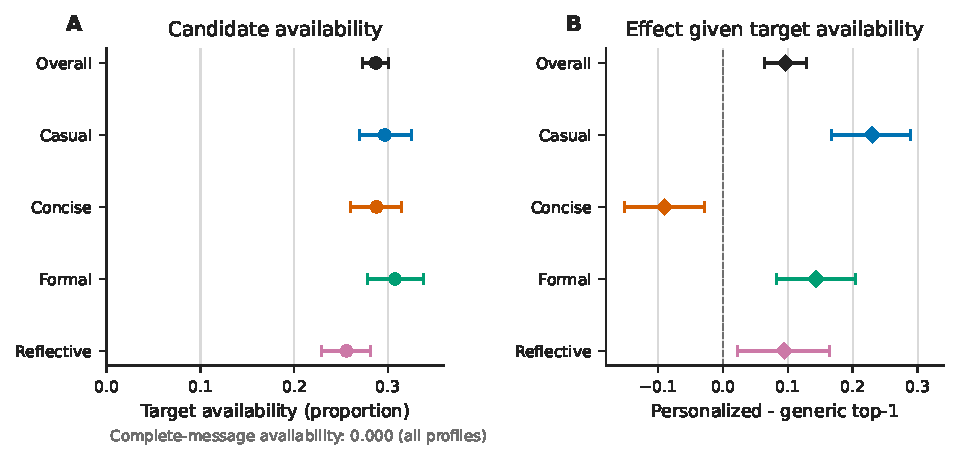
\includegraphics[width=0.98\linewidth]{figures/figure-1-language-bottleneck.pdf}
\caption{Frozen language availability and conditional personalization. Primary synthetic-language evidence. (A) Exact target availability with 95\% message-clustered bootstrap intervals. (B) Paired personalized-minus-generic top-1 difference conditional on availability. The concise profile is the only profile with a clearly negative conditional top-1 difference. Complete-message availability was zero.}
\label{fig:figure-1-language-bottleneck}
\end{figure}
\clearpage

\clearpage
\begin{landscape}
\begin{table}[H]
\centering
\caption{Frozen held-out language availability and personalization. Primary synthetic-language evidence. Top-1 rates marked "all" include unavailable targets as failures. Paired deltas and MRR are conditional on target availability; 95\% intervals resample complete messages within fixed profile strata.}
\label{tab:table-2-language-primary}
\scriptsize
\setlength{\tabcolsep}{3.5pt}
\renewcommand{\arraystretch}{1.15}
\resizebox{\linewidth}{!}{%
\begin{tabular}{@{}llllllllll@{}}
\toprule
\textbf{Profile} & \textbf{Spans} & \textbf{Target available} & \textbf{Availability 95\% CI} & \textbf{Generic top-1 (all)} & \textbf{Personalized top-1 (all)} & \textbf{Top-1 delta given available (95\% CI)} & \textbf{Generic MRR given available} & \textbf{Personalized MRR given available} & \textbf{MRR delta given available (95\% CI)} \\
\midrule
Overall & 3990 & 0.287 & [0.273, 0.301] & 0.041 & 0.068 & +0.096 [+0.064, +0.129] & 0.350 & 0.436 & +0.087 [+0.063, +0.112] \\
Casual & 998 & 0.297 & [0.269, 0.325] & 0.023 & 0.091 & +0.230 [+0.168, +0.288] & 0.288 & 0.487 & +0.199 [+0.152, +0.243] \\
Concise & 997 & 0.288 & [0.260, 0.315] & 0.065 & 0.039 & -0.091 [-0.152, -0.029] & 0.400 & 0.368 & -0.033 [-0.078, +0.013] \\
Formal & 998 & 0.308 & [0.279, 0.338] & 0.036 & 0.080 & +0.143 [+0.082, +0.205] & 0.365 & 0.459 & +0.094 [+0.048, +0.140] \\
Reflective & 997 & 0.256 & [0.229, 0.282] & 0.038 & 0.062 & +0.094 [+0.022, +0.164] & 0.346 & 0.428 & +0.082 [+0.023, +0.139] \\
\bottomrule
\end{tabular}%
}
\vspace{2pt}
\begin{minipage}{0.98\linewidth}
\footnotesize\textit{Evidence role: primary. Source: checksum-verified publication display.}
\end{minipage}
\end{table}
\end{landscape}
\clearpage

\subsection{Held-out original-task P300 decoding}

Both decoders were evaluated on \textbf{21,491 labeled test epochs} from three held-out participants. xDAWN-LDA achieved \textbf{AUROC 0.800}, balanced accuracy 0.586, \textbf{Brier 0.062}, and ECE 0.017. At the selection-trial level, its target-event recall at the known target count was \textbf{0.355 [95\% CI 0.291, 0.423]}, target-event average precision was 0.396 [0.322, 0.459], and the top event was a target in 0.560 [0.421, 0.694] of selections. Exact recovery of the complete occurrence-level target-event set was 0.009 [0.000, 0.032], illustrating the stringency of that outcome.


EEGNet produced a similar AUROC of 0.802 and higher balanced accuracy of 0.731, but its Brier score was 0.152 and ECE was 0.218. Paired selection contrasts for target-event recall, average precision, and top-event hit all had intervals spanning zero. The EEGNet-minus-xDAWN Brier difference was \textbf{+0.089 [95\% CI +0.084, +0.095]}, where a positive value is worse. The comparator therefore did not establish a selection-ranking advantage and was substantially less well calibrated under the locked recipes.


\begin{figure}[p]
\centering
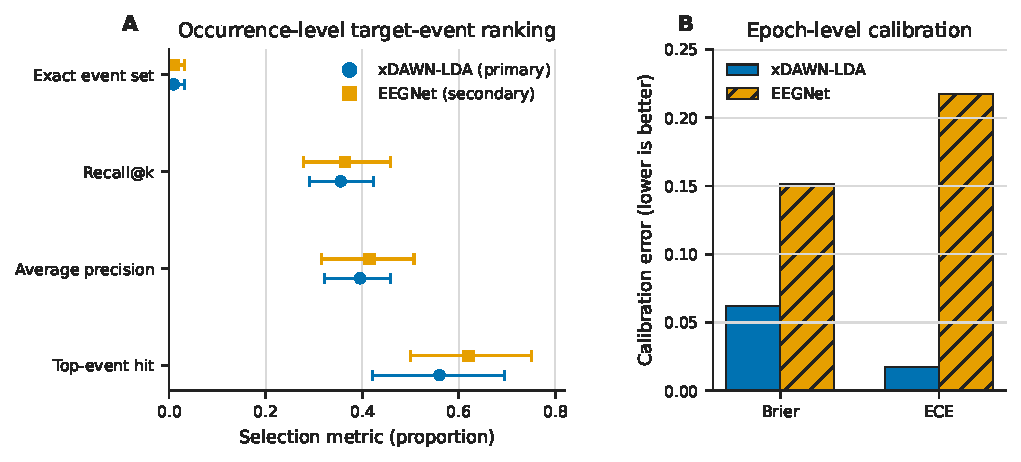
\includegraphics[width=0.98\linewidth]{figures/figure-2-p300-comparison.pdf}
\caption{Original-task P300 decoder evidence. Original-task public-EEG evidence. (A) xDAWN-LDA and the secondary EEGNet comparator with held-out-subject then selection-trial 95\% intervals. Paired intervals for the three ranking differences included zero. (B) Epoch-level Brier score and expected calibration error; lower is better. EEGNet had substantially worse calibration.}
\label{fig:figure-2-p300-comparison}
\end{figure}
\clearpage

\clearpage
\begin{landscape}
\begin{table}[H]
\centering
\caption{Held-out original-task Study P decoder performance. Original-task public-EEG evidence over 21,491 held-out labeled epochs from three subjects. Selection intervals use a held-out-subject then selection-trial bootstrap. Selection metrics concern occurrence-level target events, not NeuroSelect symbols.}
\label{tab:table-3-p300-original-task}
\scriptsize
\setlength{\tabcolsep}{3.5pt}
\renewcommand{\arraystretch}{1.15}
\resizebox{\linewidth}{!}{%
\begin{tabular}{@{}lllllllllll@{}}
\toprule
\textbf{Model} & \textbf{Role} & \textbf{Labeled epochs} & \textbf{AUROC} & \textbf{Balanced accuracy} & \textbf{Brier} & \textbf{ECE} & \textbf{Exact event set (95\% CI)} & \textbf{Target-event recall@k (95\% CI)} & \textbf{Target-event AP (95\% CI)} & \textbf{Top-event hit (95\% CI)} \\
\midrule
xDAWN-LDA & Primary decoder & 21491 & 0.800 & 0.586 & 0.062 & 0.017 & 0.009 [0.000, 0.032] & 0.355 [0.291, 0.423] & 0.396 [0.322, 0.459] & 0.560 [0.421, 0.694] \\
EEGNet & Secondary comparator & 21491 & 0.802 & 0.731 & 0.152 & 0.218 & 0.009 [0.000, 0.032] & 0.364 [0.278, 0.458] & 0.415 [0.315, 0.507] & 0.620 [0.500, 0.750] \\
\bottomrule
\end{tabular}%
}
\vspace{2pt}
\begin{minipage}{0.98\linewidth}
\footnotesize\textit{Evidence role: primary-with-secondary-comparator. Source: checksum-verified publication display.}
\end{minipage}
\end{table}
\end{landscape}
\clearpage

\begin{table}[H]
\centering
\caption{Paired EEGNet-minus-xDAWN selection contrasts. Secondary model comparison on identical held-out subjects and selection trials. Intervals crossing zero do not establish a selection-ranking difference; the strictly positive Brier contrast indicates worse EEGNet calibration.}
\label{tab:table-3b-p300-paired-contrasts}
\scriptsize
\setlength{\tabcolsep}{3.5pt}
\renewcommand{\arraystretch}{1.15}
\resizebox{\linewidth}{!}{%
\begin{tabular}{@{}llll@{}}
\toprule
\textbf{Metric} & \textbf{EEGNet - xDAWN} & \textbf{95\% CI} & \textbf{Sampling unit} \\
\midrule
Exact target-event set & +0.000 & [+0.000, +0.000] & paired\_held\_out\_subject\_then\_selection\_trial \\
Target-event recall@k & +0.009 & [-0.020, +0.040] & paired\_held\_out\_subject\_then\_selection\_trial \\
Target-event average precision & +0.019 & [-0.010, +0.053] & paired\_held\_out\_subject\_then\_selection\_trial \\
Top-event hit & +0.060 & [-0.014, +0.139] & paired\_held\_out\_subject\_then\_selection\_trial \\
Brier (positive is worse) & +0.089 & [+0.084, +0.095] & paired\_held\_out\_subject\_then\_selection\_trial \\
\bottomrule
\end{tabular}%
}
\vspace{2pt}
\begin{minipage}{0.98\linewidth}
\footnotesize\textit{Evidence role: primary-with-secondary-comparator. Source: checksum-verified publication display.}
\end{minipage}
\end{table}

\subsection{Counterfactual fusion}

Target availability in the balanced replay was \textbf{0.271 in every condition}, making the coverage ceiling visible rather than excluding unavailable trials. BCI-only replay achieved top-1 recall and completion of 0.250. Generic language alone achieved 0.042 for both outcomes. Neural plus language and neural plus personalized language each achieved 0.250. Adding retrieval raised top-1 recall and completion to 0.257.


The complete system achieved top-1 recall 0.257, completion 0.250, and repeat-request rate 0.042. Relative to BCI-only replay, its paired top-1 difference was \textbf{+0.007 [95\% CI +0.000, +0.028]}, while its completion difference was \textbf{+0.000 [95\% CI +0.000, +0.000]}. The safety policy did not change top-1 recall, reduced completion by 0.007, and increased repeat requests by 0.042. These results do not demonstrate an end-to-end advantage for the complete configuration.


\begin{figure}[p]
\centering
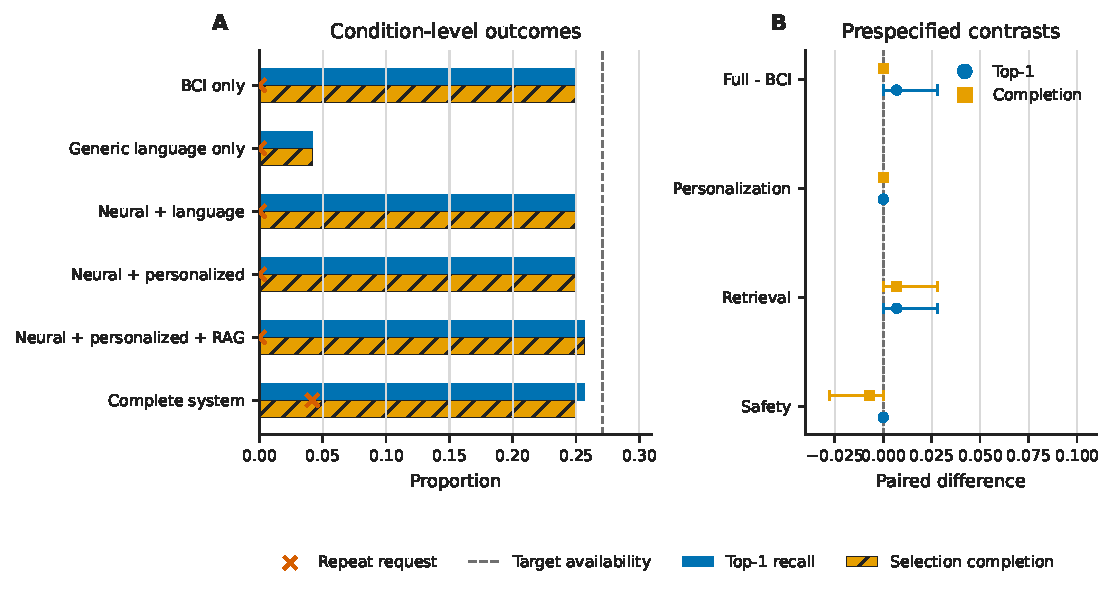
\includegraphics[width=0.98\linewidth]{figures/figure-3-counterfactual-fusion.pdf}
\caption{Offline counterfactual fusion outcomes. Primary counterfactual-replay evidence. (A) Outcomes for the six prespecified conditions; the dashed line is target availability, not a performance target. (B) Paired 95\% intervals from resampling complete messages within held-out subjects. The complete system did not improve completion over BCI-only replay.}
\label{fig:figure-3-counterfactual-fusion}
\end{figure}
\clearpage

\begin{table}[H]
\centering
\caption{Offline counterfactual fusion conditions. Primary counterfactual-replay evidence. Each condition contains 144 balanced trials from three held-out EEG subjects. Recorded P300 evidence was remapped to synthetic candidate menus; these are not live communication outcomes.}
\label{tab:table-4-counterfactual-conditions}
\scriptsize
\setlength{\tabcolsep}{3.5pt}
\renewcommand{\arraystretch}{1.15}
\resizebox{\linewidth}{!}{%
\begin{tabular}{@{}llllll@{}}
\toprule
\textbf{Condition} & \textbf{Condition trials} & \textbf{Target available} & \textbf{Top-1 recall} & \textbf{Selection completion} & \textbf{Repeat request} \\
\midrule
BCI only & 144 & 0.271 & 0.250 & 0.250 & 0.000 \\
Generic language only & 144 & 0.271 & 0.042 & 0.042 & 0.000 \\
Neural + language & 144 & 0.271 & 0.250 & 0.250 & 0.000 \\
Neural + personalized & 144 & 0.271 & 0.250 & 0.250 & 0.000 \\
Neural + personalized + RAG & 144 & 0.271 & 0.257 & 0.257 & 0.000 \\
Complete system & 144 & 0.271 & 0.257 & 0.250 & 0.042 \\
\bottomrule
\end{tabular}%
}
\vspace{2pt}
\begin{minipage}{0.98\linewidth}
\footnotesize\textit{Evidence role: primary. Source: checksum-verified publication display.}
\end{minipage}
\end{table}

\begin{table}[H]
\centering
\caption{Prespecified paired counterfactual contrasts. Paired differences resample complete messages within held-out EEG subjects. The complete system did not improve completion over BCI-only replay.}
\label{tab:table-4b-counterfactual-contrasts}
\scriptsize
\setlength{\tabcolsep}{3.5pt}
\renewcommand{\arraystretch}{1.15}
\resizebox{\linewidth}{!}{%
\begin{tabular}{@{}lllll@{}}
\toprule
\textbf{Contrast} & \textbf{Metric} & \textbf{Difference} & \textbf{95\% CI} & \textbf{Sampling unit} \\
\midrule
Complete system - BCI only & Top-1 recall & +0.007 & [+0.000, +0.028] & held\_out\_subject\_then\_complete\_message \\
Complete system - BCI only & Selection completion & +0.000 & [+0.000, +0.000] & held\_out\_subject\_then\_complete\_message \\
Neural personalized - neural language & Top-1 recall & +0.000 & [+0.000, +0.000] & held\_out\_subject\_then\_complete\_message \\
Neural personalized - neural language & Selection completion & +0.000 & [+0.000, +0.000] & held\_out\_subject\_then\_complete\_message \\
Add retrieval context & Top-1 recall & +0.007 & [+0.000, +0.028] & held\_out\_subject\_then\_complete\_message \\
Add retrieval context & Selection completion & +0.007 & [+0.000, +0.028] & held\_out\_subject\_then\_complete\_message \\
Add safety policy & Top-1 recall & +0.000 & [+0.000, +0.000] & held\_out\_subject\_then\_complete\_message \\
Add safety policy & Selection completion & -0.007 & [-0.028, +0.000] & held\_out\_subject\_then\_complete\_message \\
Add safety policy & Repeat request & +0.042 & [+0.000, +0.097] & held\_out\_subject\_then\_complete\_message \\
\bottomrule
\end{tabular}%
}
\vspace{2pt}
\begin{minipage}{0.98\linewidth}
\footnotesize\textit{Evidence role: primary. Source: checksum-verified publication display.}
\end{minipage}
\end{table}

\subsection{Exploratory target-blind candidate generation}

On the existing test-exposed benchmark, full v2 generation increased exact-span availability from 0.287 to \textbf{0.525}, a paired difference of \textbf{+0.238 [95\% CI +0.219, +0.257]}. Complete-message availability rose from 0.000 to 0.021. Removing grammar routing reduced span availability to 0.129; removing profile conditioning reduced it to 0.473. Frequency-only retrieval reached 0.471. These comparisons indicate that the grammar route made the largest contribution on the exposed benchmark, but they are exploratory and not a replacement for the frozen result.


The two-stage opening interface reached span availability 0.560, opening availability 0.188, and complete-message availability 0.091 on the existing benchmark. On the locked held-out-combination benchmark, one-stage full v2 had \textbf{0.000 opening availability}, while two-stage composition had \textbf{1.000 opening availability} and 0.323 complete-message availability. The gain required a mean of 1.250 reached stages rather than one stage. Because the stems and actions were individually observed and the benchmark was developer-authored, complete opening coverage is evidence of constrained composition only.


\begin{figure}[p]
\centering
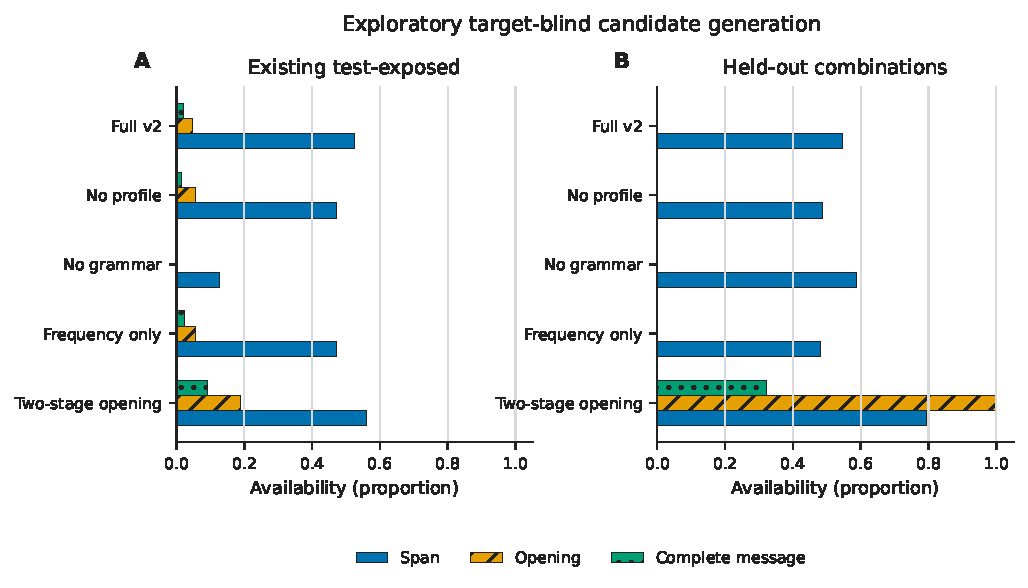
\includegraphics[width=0.98\linewidth]{figures/figure-4-candidate-generation.pdf}
\caption{Exploratory candidate-generation ablations and robustness. Exploratory synthetic evidence at a nine-candidate budget. (A) Existing benchmark that was exposed during development. (B) Exact stem-action combinations held out before Step 4 execution. The two-stage interface improves opening and complete-message availability but adds a selection stage.}
\label{fig:figure-4-candidate-generation}
\end{figure}
\clearpage

\begin{table}[H]
\centering
\caption{Exploratory target-blind candidate availability. Exploratory synthetic evidence at a nine-candidate menu budget. The existing benchmark was inspected during v2 development; the held-out-combination benchmark was locked before Step 4 execution. Intended targets were used only after generation for scoring.}
\label{tab:table-5-candidate-generation}
\scriptsize
\setlength{\tabcolsep}{3.5pt}
\renewcommand{\arraystretch}{1.15}
\resizebox{\linewidth}{!}{%
\begin{tabular}{@{}llllll@{}}
\toprule
\textbf{Dataset} & \textbf{Method} & \textbf{Span availability} & \textbf{Opening availability} & \textbf{Complete-message availability} & \textbf{Mean planned/reached stages} \\
\midrule
Existing test-exposed & Frozen v1 reference & 0.287 & 0.000 & 0.000 & 1.000 \\
Existing test-exposed & Full v2 & 0.525 & 0.048 & 0.021 & 1.000 \\
Existing test-exposed & No profile & 0.473 & 0.057 & 0.014 & 1.000 \\
Existing test-exposed & No grammar & 0.129 & 0.000 & 0.000 & 1.000 \\
Existing test-exposed & Frequency only & 0.471 & 0.057 & 0.023 & 1.000 \\
Existing test-exposed & Two-stage opening & 0.560 & 0.188 & 0.091 & 1.251 \\
Held-out combinations & Full v2 & 0.545 & 0.000 & 0.000 & 1.000 \\
Held-out combinations & No profile & 0.487 & 0.000 & 0.000 & 1.000 \\
Held-out combinations & No grammar & 0.588 & 0.000 & 0.000 & 1.000 \\
Held-out combinations & Frequency only & 0.480 & 0.000 & 0.000 & 1.000 \\
Held-out combinations & Two-stage opening & 0.795 & 1.000 & 0.323 & 1.250 \\
\bottomrule
\end{tabular}%
}
\vspace{2pt}
\begin{minipage}{0.98\linewidth}
\footnotesize\textit{Evidence role: exploratory. Source: checksum-verified publication display.}
\end{minipage}
\end{table}

\begin{table}[H]
\centering
\caption{Selected paired candidate-generation contrasts. Paired 10,000-resample intervals over complete messages within fixed synthetic profile strata. Step 3 v2 comparisons are test-exposed; Step 4 comparisons were locked before execution.}
\label{tab:table-5b-candidate-contrasts}
\scriptsize
\setlength{\tabcolsep}{3.5pt}
\renewcommand{\arraystretch}{1.15}
\resizebox{\linewidth}{!}{%
\begin{tabular}{@{}llll@{}}
\toprule
\textbf{Dataset} & \textbf{Contrast} & \textbf{Difference} & \textbf{95\% CI} \\
\midrule
Existing test-exposed & v2 - frozen v1, spans & +0.238 & [+0.219, +0.257] \\
Existing test-exposed & v2 - frozen v1, complete messages & +0.021 & [+0.013, +0.030] \\
Existing test-exposed & full v2-minus-no profile conditioning-overall & +0.052 & [+0.042, +0.062] \\
Existing test-exposed & full v2-minus-no grammar routing-overall & +0.396 & [+0.385, +0.407] \\
Existing test-exposed & two stage opening-minus-full v2-overall & +0.035 & [+0.030, +0.040] \\
Existing test-exposed & two stage opening-minus-full v2-opening & +0.140 & [+0.121, +0.160] \\
Existing test-exposed & two stage opening-minus-full v2-complete messages & +0.070 & [+0.055, +0.085] \\
Held-out combinations & full v2-minus-no profile conditioning-overall & +0.059 & [+0.046, +0.071] \\
Held-out combinations & full v2-minus-no grammar routing-overall & -0.043 & [-0.053, -0.032] \\
Held-out combinations & two stage opening-minus-full v2-overall & +0.250 & [+0.250, +0.250] \\
Held-out combinations & two stage opening-minus-full v2-opening & +1.000 & [+1.000, +1.000] \\
Held-out combinations & two stage opening-minus-full v2-complete messages & +0.323 & [+0.294, +0.352] \\
\bottomrule
\end{tabular}%
}
\vspace{2pt}
\begin{minipage}{0.98\linewidth}
\footnotesize\textit{Evidence role: exploratory. Source: checksum-verified publication display.}
\end{minipage}
\end{table}

\subsection{Exploratory hierarchical openings}

On 288 held-out stem/content combinations, one-stage phrase retrieval had \textbf{0.000 availability}, two-stage stem/content composition reached \textbf{0.250}, and three-stage intent/stem/content composition reached \textbf{0.667}. Coverage per required selection was 0.000, 0.125, and 0.222, respectively. The three-stage method reached three menus and exposed a mean of 19 candidates, so its coverage gain carried explicit interaction cost.


On 384 openings whose paraphrase-family stems were absent from fitting, \textbf{all three methods had 0.000 availability}. Two-stage composition failed at the unseen stem; three-stage composition could select an intent but still failed to supply the required stem. The hierarchy therefore combined observed components but did not provide open-vocabulary generation.


\begin{figure}[p]
\centering
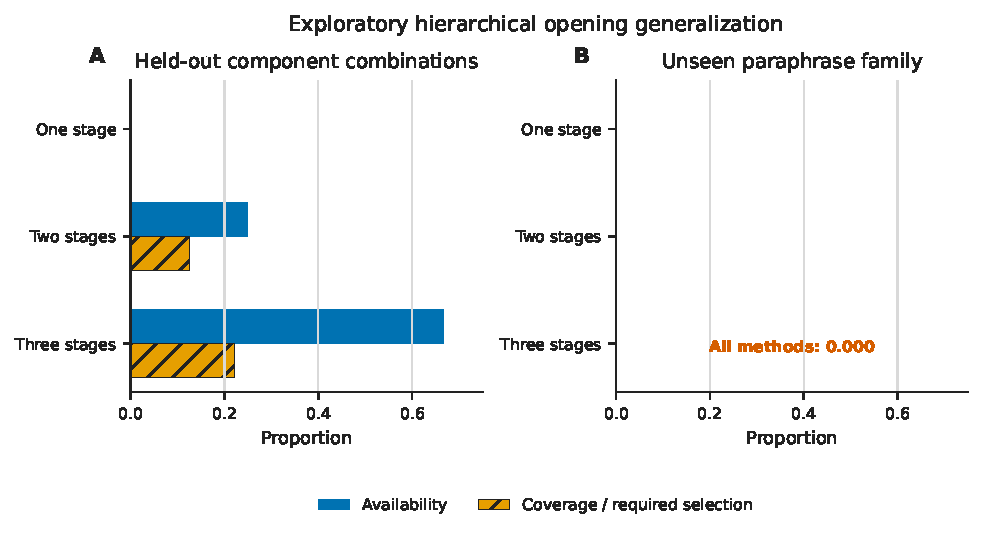
\includegraphics[width=0.98\linewidth]{figures/figure-5-opening-generalization.pdf}
\caption{Hierarchical opening composition and closed-vocabulary boundary. Locked exploratory synthetic evidence. Availability and availability per planned selection are shown for (A) unseen combinations of observed components and (B) paraphrase-family stems absent from fitting. Hierarchy improved composition of observed components but every method failed on unseen surface families.}
\label{fig:figure-5-opening-generalization}
\end{figure}
\clearpage

\clearpage
\begin{landscape}
\begin{table}[H]
\centering
\caption{Locked hierarchical opening-generalization results. Exploratory target-blind opening evidence under a maximum menu size of nine. Combination tests contain unseen exact pairs of observed components; paraphrase-family tests contain stems absent from fitting. Downstream menus use only simulated observed selections.}
\label{tab:table-6-opening-generalization}
\scriptsize
\setlength{\tabcolsep}{3.5pt}
\renewcommand{\arraystretch}{1.15}
\resizebox{\linewidth}{!}{%
\begin{tabular}{@{}llllllll@{}}
\toprule
\textbf{Challenge} & \textbf{Method} & \textbf{Openings} & \textbf{Availability} & \textbf{Planned selections} & \textbf{Coverage per required selection} & \textbf{Mean menus reached} & \textbf{Mean candidate exposures} \\
\midrule
Held-out stem/content combinations & One-stage phrase & 288 & 0.000 & 1 & 0.000 & 1.000 & 9.000 \\
Held-out stem/content combinations & Two-stage stem/content & 288 & 0.250 & 2 & 0.125 & 1.375 & 12.375 \\
Held-out stem/content combinations & Three-stage intent/stem/content & 288 & 0.667 & 3 & 0.222 & 3.000 & 19.000 \\
Unseen paraphrase family & One-stage phrase & 384 & 0.000 & 1 & 0.000 & 1.000 & 9.000 \\
Unseen paraphrase family & Two-stage stem/content & 384 & 0.000 & 2 & 0.000 & 1.000 & 9.000 \\
Unseen paraphrase family & Three-stage intent/stem/content & 384 & 0.000 & 3 & 0.000 & 2.000 & 10.000 \\
\bottomrule
\end{tabular}%
}
\vspace{2pt}
\begin{minipage}{0.98\linewidth}
\footnotesize\textit{Evidence role: exploratory. Source: checksum-verified publication display.}
\end{minipage}
\end{table}
\end{landscape}
\clearpage

\begin{table}[H]
\centering
\caption{Paired hierarchical opening contrasts. Paired 10,000-resample intervals over openings within fixed synthetic-profile strata. Zero availability for every unseen-family method is retained rather than omitted.}
\label{tab:table-6b-opening-contrasts}
\scriptsize
\setlength{\tabcolsep}{3.5pt}
\renewcommand{\arraystretch}{1.15}
\resizebox{\linewidth}{!}{%
\begin{tabular}{@{}lllll@{}}
\toprule
\textbf{Challenge} & \textbf{Metric} & \textbf{Contrast} & \textbf{Difference} & \textbf{95\% CI} \\
\midrule
Held-out combinations & availability rate & Two-stage stem/content - One-stage phrase & +0.250 & [+0.201, +0.299] \\
Held-out combinations & availability rate & Three-stage intent/stem/content - One-stage phrase & +0.667 & [+0.615, +0.722] \\
Held-out combinations & availability rate & Three-stage intent/stem/content - Two-stage stem/content & +0.417 & [+0.361, +0.476] \\
Held-out combinations & coverage per required selection & Two-stage stem/content - One-stage phrase & +0.125 & [+0.101, +0.151] \\
Held-out combinations & coverage per required selection & Three-stage intent/stem/content - One-stage phrase & +0.222 & [+0.204, +0.241] \\
Held-out combinations & coverage per required selection & Three-stage intent/stem/content - Two-stage stem/content & +0.097 & [+0.073, +0.121] \\
Unseen paraphrase family & availability rate & Two-stage stem/content - One-stage phrase & +0.000 & [+0.000, +0.000] \\
Unseen paraphrase family & availability rate & Three-stage intent/stem/content - One-stage phrase & +0.000 & [+0.000, +0.000] \\
Unseen paraphrase family & availability rate & Three-stage intent/stem/content - Two-stage stem/content & +0.000 & [+0.000, +0.000] \\
Unseen paraphrase family & coverage per required selection & Two-stage stem/content - One-stage phrase & +0.000 & [+0.000, +0.000] \\
Unseen paraphrase family & coverage per required selection & Three-stage intent/stem/content - One-stage phrase & +0.000 & [+0.000, +0.000] \\
Unseen paraphrase family & coverage per required selection & Three-stage intent/stem/content - Two-stage stem/content & +0.000 & [+0.000, +0.000] \\
\bottomrule
\end{tabular}%
}
\vspace{2pt}
\begin{minipage}{0.98\linewidth}
\footnotesize\textit{Evidence role: exploratory. Source: checksum-verified publication display.}
\end{minipage}
\end{table}

\section{Discussion}

\subsection{Principal findings}

The main result is a bottleneck decomposition rather than a claim of complete-system efficacy. First, the frozen target-blind generator made intended spans available in fewer than one third of rounds and never covered an entire held-out message. Second, profile adapters improved average conditional ranking, but the effect was not uniform and the concise profile worsened on conditional top-1 recall. Third, the primary xDAWN-LDA decoder discriminated original-task target events with an AUROC of 0.800 and lower Brier score and ECE than EEGNet, whereas EEGNet did not establish a paired selection-ranking advantage. Fourth, counterfactual fusion did not improve completion over BCI-only replay. Finally, exploratory hierarchy improved composition when every component had been observed, yet every tested method failed on unseen paraphrase families.


Taken together, these findings show why component separation matters. Reporting only conditional personalized ranking would emphasize a positive average effect while hiding the 28.7\% candidate ceiling and 0\% complete-message coverage. Reporting only EEG AUROC would hide the much lower exact target-event-set recovery. Reporting only the best exploratory hierarchy would hide its additional selections, developer-authored vocabulary, and complete failure on unseen families.


\subsection{Candidate availability precedes ranking}

Phrase ranking and candidate construction are sequential constraints. The ranker can affect which visible item appears first but cannot recover an absent target. In NeuroSelect, personalization was applied only after a fixed set was created, so its average conditional benefit did not change availability. This design exposes the distinction cleanly and suggests that future work should prioritize candidate recall under a realistic menu and interaction budget before investing in more complex rankers.


The exploratory v2 result demonstrates that availability is changeable: grammar routing and profile-aware retrieval approximately doubled span coverage on the existing benchmark. It also shows why this is not yet a solved problem. Complete-message coverage remained low, the benchmark was exposed during development, and the robustness sources were synthetic and developer-authored. The hierarchy then clarified what compositional menus can and cannot do. They reduce the combinatorial burden for known stems and contents, but they do not invent an unseen surface family.


An open-vocabulary system would require a mechanism that can generate or spell a missing component rather than only retrieve it from a fitted bank. Plausible next designs include a hybrid menu with an explicit character-level fallback, constrained subword generation, semantic retrieval over a larger user-controlled lexicon, or a generative opening stage with conservative confirmation. Those alternatives should be evaluated on an independently authored benchmark with lexical-family holdout and measured selection cost. Intended targets must remain unavailable to the generator at inference.


\subsection{Personalization is heterogeneous}

The overall conditional ranking improvement supports the narrower statement that profile-specific adapters changed ordering on the frozen synthetic benchmark. It does not imply a universal personalization benefit. The concise profile's negative conditional top-1 effect is especially important because a system optimized only for the pooled mean could reduce performance in a controlled style condition.


Several mechanisms could produce this pattern. Concise messages provide shorter contexts and may leave fewer style cues for an adapter. The adapter may increase likelihood for generally concise candidates that differ from the exact held-out span. Mean-token log likelihood can also favor different phrase lengths or lexical choices. Because profiles are synthetic, the result is a controlled model-behavior finding rather than a claim about user groups. A future participant-free study could test adapter stability across seeds, corpus sizes, and independently authored profiles, and could report semantic acceptability alongside exact-span recall.


\subsection{Neural evidence and probability calibration}

The original-task analysis supports using the xDAWN-LDA probabilities as a transparent offline neural evidence source. It does not support calling 0.800 AUROC a word or message accuracy. Selection trials contain multiple target occurrences, and exact event-set recovery was deliberately strict. The large gap between epoch AUROC and exact set recovery illustrates how apparently strong binary discrimination can translate into a much harder structured selection problem.


EEGNet's balanced accuracy was higher, but its paired selection-ranking intervals crossed zero and its probabilities were much less calibrated. A fusion system needs meaningful relative evidence, not merely a thresholded class decision. xDAWN-LDA had been prespecified as the primary decoder; EEGNet was added later as a locked comparator rather than used for post-test model selection. Its calibration result therefore informs interpretation and future model choice, not the choice of the reported primary model. Broader conclusions would require more held-out participants, repeated training seeds, and possibly nested cross-validation. The current test set contains three participants, so participant-level uncertainty remains substantial.


\subsection{What counterfactual replay establishes}

Counterfactual replay is useful because it exercises the implemented candidate and fusion path with recorded neural probabilities and explicit provenance. It can reveal policy behavior, unavailable targets, and contrasts between scoring conditions. Here it showed that adding personalization did not change the selected item in the balanced sample, retrieval produced only a small top-1 change, and the safety layer converted some selections into repeat requests without improving completion.


Replay cannot establish that a person could attend to the remapped tiles, that the neural response would remain unchanged under a different display, or that the resulting phrase expresses the participant's intent. The source participants selected characters in the Study P task. They did not author the synthetic messages or use NeuroSelect. A live or clinical claim would require a new protocol, ethics review, consent, real interface exposure, usability outcomes, and comparison with established augmentative and alternative communication options.


\subsection{Reproducibility contribution}

The framework's methodological contribution is its fail-closed evidence chain. Data selection, participant splits, preprocessing, model recipes, language adapters, replay mappings, statistical resampling, tables, figures, manuscript claims, and document assembly all carry machine-readable identity. The pipeline refuses unverified source replacement and records whether the source tree was clean. This does not make the scientific conclusions stronger than their samples, but it makes the limits and transformations inspectable.


The manuscript itself is assembled from the same display bundle used for exact CSV tables and 300-dpi/vector figures. A claim ledger verifies the principal quantitative phrases against source cells or tracked configuration values. External submission gates remain separate: a clean build does not substitute for institutional secondary-use wording, open-access confirmation, scientific review, or final author metadata.


\subsection{Limitations}

The study has eight main limitations. First, language profiles and messages are synthetic; exact-span metrics can penalize semantically acceptable alternatives, while controlled language may underrepresent natural communication. Second, the primary language protocol is retrospective and the v2 benchmark was exposed during development. The later robustness experiments were locked before execution but remain developer-authored.


Third, Study P measures an original predictive/non-predictive spelling task. Predictive and non-predictive condition order varies across the source design, so session differences cannot be attributed solely to time or electrode drift. Only three participants were held out for test, and the EEG results do not represent NeuroSelect phrase selection. Fourth, counterfactual replay preserves recorded evidence but changes the displayed interpretation; it is not a substitute for live data.


Fifth, lexical retrieval and tracked safety tags are intentionally narrow. They do not constitute a semantic memory system, a general content-safety classifier, or a clinical safeguard. Sixth, the hierarchical opening experiments teacher-force simulated correct intermediate selections and report planned selection cost rather than measured interaction time, fatigue, visual load, or error correction. Seventh, each LoRA adapter and EEGNet were trained with one fixed seed, and generation was evaluated as one frozen realization. The bootstrap intervals therefore do not represent training- or generation-induced variability. Eighth, primary next-span evaluation teacher-forced the reference history, so it does not measure cascading errors during autonomous message construction.


\section{Conclusions}

NeuroSelect is a reproducible offline framework for studying profile-conditioned language ranking and counterfactual P300 candidate fusion while preserving evidence boundaries. In the frozen evaluation, low target availability and zero complete-message availability constrained the language path. Personalization improved conditional ranking on average but reduced one profile-level top-1 outcome. The prespecified calibrated xDAWN-LDA decoder achieved an original-task AUROC of 0.800. The secondary EEGNet comparator did not establish a selection-ranking advantage, and counterfactual full fusion did not establish a completion advantage over BCI-only replay.


Exploratory compositional menus improved coverage for new combinations of observed parts and made message openings a tractable object of study. Their failure on every unseen paraphrase family defines the next technical question: how to introduce a verified generative or spelling fallback without hiding added selections, unsafe attribution, or target leakage. The present evidence supports an offline computational methods paper, not a claim of live communication or clinical benefit.


\section*{Declarations}

\addcontentsline{toc}{section}{Declarations}

\subsection{Data and code availability}

Source code, tracked protocols, synthetic benchmark sources, tests, and manuscript sources will be released at \url{https://github.com/NickSomitsch/neuroselect-bci} under the MIT License before submission. Study P is available separately from PhysioNet under CC BY 4.0 \cite{mainsah2025}. Raw EEG, cached base-model weights, trained adapters, and other license-controlled local artifacts will not be redistributed in the source repository. Each reported run records source and output digests needed to verify local artifacts; non-restricted result manifests, tables, figures, and publication-analysis outputs will accompany the public release.


\subsection{Ethics statement}

This work recruited no participants and performed no live NeuroSelect study. It used public, deidentified Study P data and synthetic language. Final journal submission remains contingent on institutionally approved wording for the secondary use of Study P; this manuscript does not independently claim an ethics exemption.


\subsection{Author contributions}

Nick Somitsch conceived and implemented the software, designed the offline experiments, performed the analyses, and drafted the manuscript. Final CRediT terminology and any additional qualifying authorship will be confirmed before submission.


\subsection{Competing interests and funding}

Competing-interest and funding declarations are external submission metadata and must be confirmed by the author before journal submission; no statement is inferred from the repository.


\bibliographystyle{unsrt}

\bibliography{references}

\end{document}
